\section{Datasets}
\label{sec:datasets}

\subsection*{GovReport}

Introduced by \citet{huang-etal-2021-efficient}, this dataset consists of 7,238 reports
written by government research agencies, including the Congressional Research Service (CRS)
and the U.S. Government Accountability Office (GAO).
Word count information is given in \autoref{tab:datasets}.
Figure \ref{fig:govreport} shows the word count distribution of the dataset.

\begin{figure}[!ht]
	\centering
	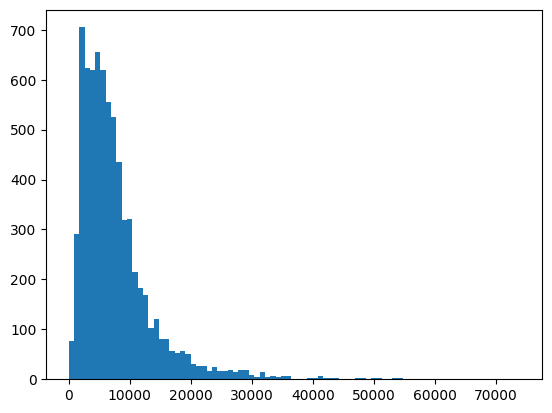
\includegraphics[width=.48\textwidth]{Images/govreport-wordcount.png}
	\caption{GovReport word counts}
	\label{fig:govreport}
\end{figure}


\subsection*{BigPatent}

Introduced in \citet{sharma-etal-2019-bigpatent}, this dataset consists of 1.3 million
records of U.S. patent documents with human wiritten abstractive summaries.
Word count information is given in \autoref{tab:datasets}.
Figure \ref{fig:bigpatent} shows the word count distribution of the dataset.

\begin{figure}[!ht]
	\centering
	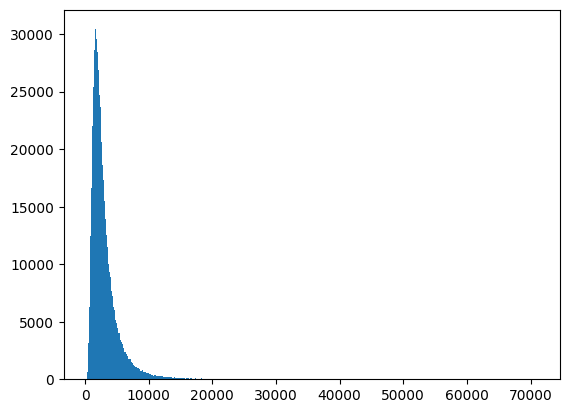
\includegraphics[width=.48\textwidth]{Images/bigpatent-wordcount.png}
	\caption{BigPatent word counts}
	\label{fig:bigpatent}
\end{figure}

\begin{table*}[!ht]
	\centering

	\begin{tabular}{c c c c}
		\hline
		\textbf{Dataset} & \textbf{Avg. Word Count} & \textbf{Max Word Count} &
		\textbf{No. of Documents} \\
		\hline
		GovReport & 7,700.71 & 73,815 & 7,238 \\
		BigPatent & 3,055.72 & 71,027 & 1,341,362 \\
		\hline
	\end{tabular}

	\caption{Dataset information}
	\label{tab:datasets}
\end{table*}
